\section{Abstract}
In this paper, we present a novel approach to solve the Set Cover problem using Grover's Algorithm, an important quantum computing algorithm known for its quadratic speed-up over classical search algorithms. The Set Cover problem is one of the most well-known NP-hard combinatorial optimization problems with a wide range of practical applications, including resource allocation, network design, and computational biology. Previous research has focused on developing heuristic and approximation algorithms with limited success due to the inherent computational complexity of the problem. Our research aims to leverage the computational power of quantum computing to provide a more efficient and scalable solution to the Set Cover problem.

\section{Introduction}
The Set Cover problem is a classical problem in computer science and mathematics, with a wide range of applications in various domains. Given a universe of elements $U$ and a collection of sets $S = \{S_1, S_2, \dots, S_m\}$, each containing a subset of elements from $U$, the goal of the Set Cover problem is to find a minimum-size subcollection of sets $C \subseteq S$ such that all elements in $U$ are covered, i.e., the union of sets in $C$ contains all elements in $U$. Formally, the problem can be defined as follows:

\begin{quote}
\emph{Input:} A universe of elements $U = \{u_1, u_2, \dots, u_n\}$ and a collection of sets $S = \{S_1, S_2, \dots, S_m\}$, where $S_i \subseteq U$ for $1 \leq i \leq m$.\\
\emph{Output:} A minimum-size subcollection of sets $C \subseteq S$ such that $\bigcup_{S_i \in C}S_i = U$.
\end{quote}

The Set Cover problem is NP-hard, which means that it is unlikely that an efficient algorithm exists to solve it exactly in the worst case. Despite its computational complexity, the problem has attracted significant research interest due to its practical relevance in many application domains, such as resource allocation, network design, and computational biology.

In recent years, quantum computing has emerged as a promising area of research with the potential to revolutionize computing by offering significant speed-up over classical algorithms for certain computational problems. One of the fundamental quantum algorithms is Grover's Algorithm, which has been shown to provide a quadratic speed-up over classical search algorithms for unsorted databases. Given a function $f: \{0,1\}^n \rightarrow \{0,1\}$, Grover's Algorithm can find an input $x$ such that $f(x) = 1$ in $O(\sqrt{N})$ steps, where $N = 2^n$ is the size of the search space.

In this paper, we present a novel approach to solving the Set Cover problem using Grover's Algorithm. Our main contribution is the development of a quantum algorithm that leverages the computational power of Grover's Algorithm to efficiently search the solution space of the Set Cover problem. We provide a detailed analysis of the algorithm's performance and discuss its practical implications for various application domains.

The rest of the paper is organized as follows. In Section 2, we provide a brief overview of Grover's Algorithm and its main properties. Section 3 describes our proposed quantum algorithm for the Set Cover problem, including a detailed explanation of the steps involved and a complexity analysis. In Section 4, we discuss potential applications of our algorithm in various domains, highlighting its practical relevance and potential impact. Finally, Section 5 concludes the paper and outlines directions for future research.

% Please add the remaining sections according to your paper content.

\section{Problem Formulation}
In the Set Cover problem, we are given a universe $U$ of elements and a collection $S$ of subsets of $U$. The objective is to find a minimum number of subsets in $S$ such that the union of these subsets covers all elements in $U$. In this particular case, we will work with a simplified version of the problem, where the largest number allowed is 3, meaning that the universe $U$ can have at most 3 distinct elements.

We represent the set of elements that need to be covered (universe $U$) in register R0 and the set of elements that are covered by the chosen subsets in register R1. Both R0 and R1 can have values ranging from 0 to 3, as each bit position represents the presence (1) or absence (0) of an element in the respective sets.

\section{Algorithm Description}
The proposed algorithm is an ARM assembly code that checks if the values in R0 and R1 are a valid solution to the Set Cover problem without using loops and branches. The algorithm follows the constraints provided and utilizes bitwise operations and available instructions to achieve the objective.

\subsection{Register Initialization}
First, the algorithm initializes two additional registers, R2 and R3, setting their values to 0. These registers will be used for temporary storage and comparisons during the execution of the algorithm.

\begin{verbatim}
MOV R2, #0
MOV R3, #0
\end{verbatim}

\subsection{Bitwise Operations}
The algorithm performs a series of bitwise operations to check if the values in R1 cover the values in R0. The first operation is a bitwise AND between R0 and R1, which is stored in R2. This operation results in a value where the bits set to 1 represent elements that are present in both R0 and R1.

\begin{verbatim}
AND R2, R0, R1
\end{verbatim}

Next, the algorithm performs a bitwise ORR operation between R0 and R1, which is stored in R3. This operation results in a value where the bits set to 1 represent elements that are present in either R0 or R1.

\begin{verbatim}
ORR R3, R0, R1
\end{verbatim}

Following that, the algorithm performs a bitwise EOR operation between R3 and R2. This operation results in a value where the bits set to 1 represent elements that are present in either R0 or R1 but not in both. This is used to check if R1 covers all elements in R0.

\begin{verbatim}
EOR R3, R3, R2
\end{verbatim}

\subsection{Setting the ZERO PSR Flag}
Lastly, the algorithm performs a bitwise AND operation (TST instruction) between R0 and R3 to set the ZERO Program Status Register (PSR) flag. The TST instruction updates the condition flags based on the result of the bitwise AND operation between its operands, without modifying the destination register. If the result of the bitwise AND operation is zero, the ZERO PSR flag is set to 1, indicating that R0 and R1 are a valid solution to the Set Cover problem. If the result is non-zero, the ZERO PSR flag is set to 0, indicating that R0 and R1 are not a valid solution.

\begin{verbatim}
TST R0, R3
\end{verbatim}

\section{Algorithm Analysis}
The proposed ARM assembly algorithm efficiently checks if the values in R0 and R1 are a valid solution to the simplified Set Cover problem without using loops, branches, or any restricted instructions. The algorithm is concise and utilizes a combination of bitwise operations and instructions to determine the validity of the solution. The algorithm's performance is constant time, as it does not depend on the size of the input values.

Although the algorithm is designed for a specific case with a limited number of elements, it demonstrates the potential for using bitwise operations and ARM assembly code to solve combinatorial problems. It can be adapted and extended to handle larger problem instances or other similar problems with additional constraints.



\section{Implementation}

The following program is an implementation of the above description. The created circuit is shown in Figure \ref{fig:Set_Cover}:

\begin{lstlisting}

{"register_size": 2, "run": false, "display": false}
HAD R0
HAD R1

ORACLE


; Initialize R2 and R3 for comparison and temporary storage
MOV R2, #0
MOV R3, #0

; Perform bitwise AND operation between R0 and R1 and store the result in R2
AND R2, R0, R1

; Perform bitwise ORR operation between R0 and R1 and store the result in R3
ORR R3, R0, R1

; Perform bitwise EOR operation between R3 and R2 to check if the values in R1 cover the values in R0
EOR R3, R3, R2

; Perform bitwise AND operation between R0 and R3 to set the ZERO PSR flag
TST R0, R3

; Now, the ZERO PSR flag will be set to 1 if R0 and R1 are a valid solution to the Set Cover problem, and 0 otherwise.



END_ORACLE

TGT ZERO

REVERSE_ORACLE

DIF {R0, R1}

STR CR0, R0
STR CR1, R1


\end{lstlisting}

\begin{figure}[htp]
    \centering
    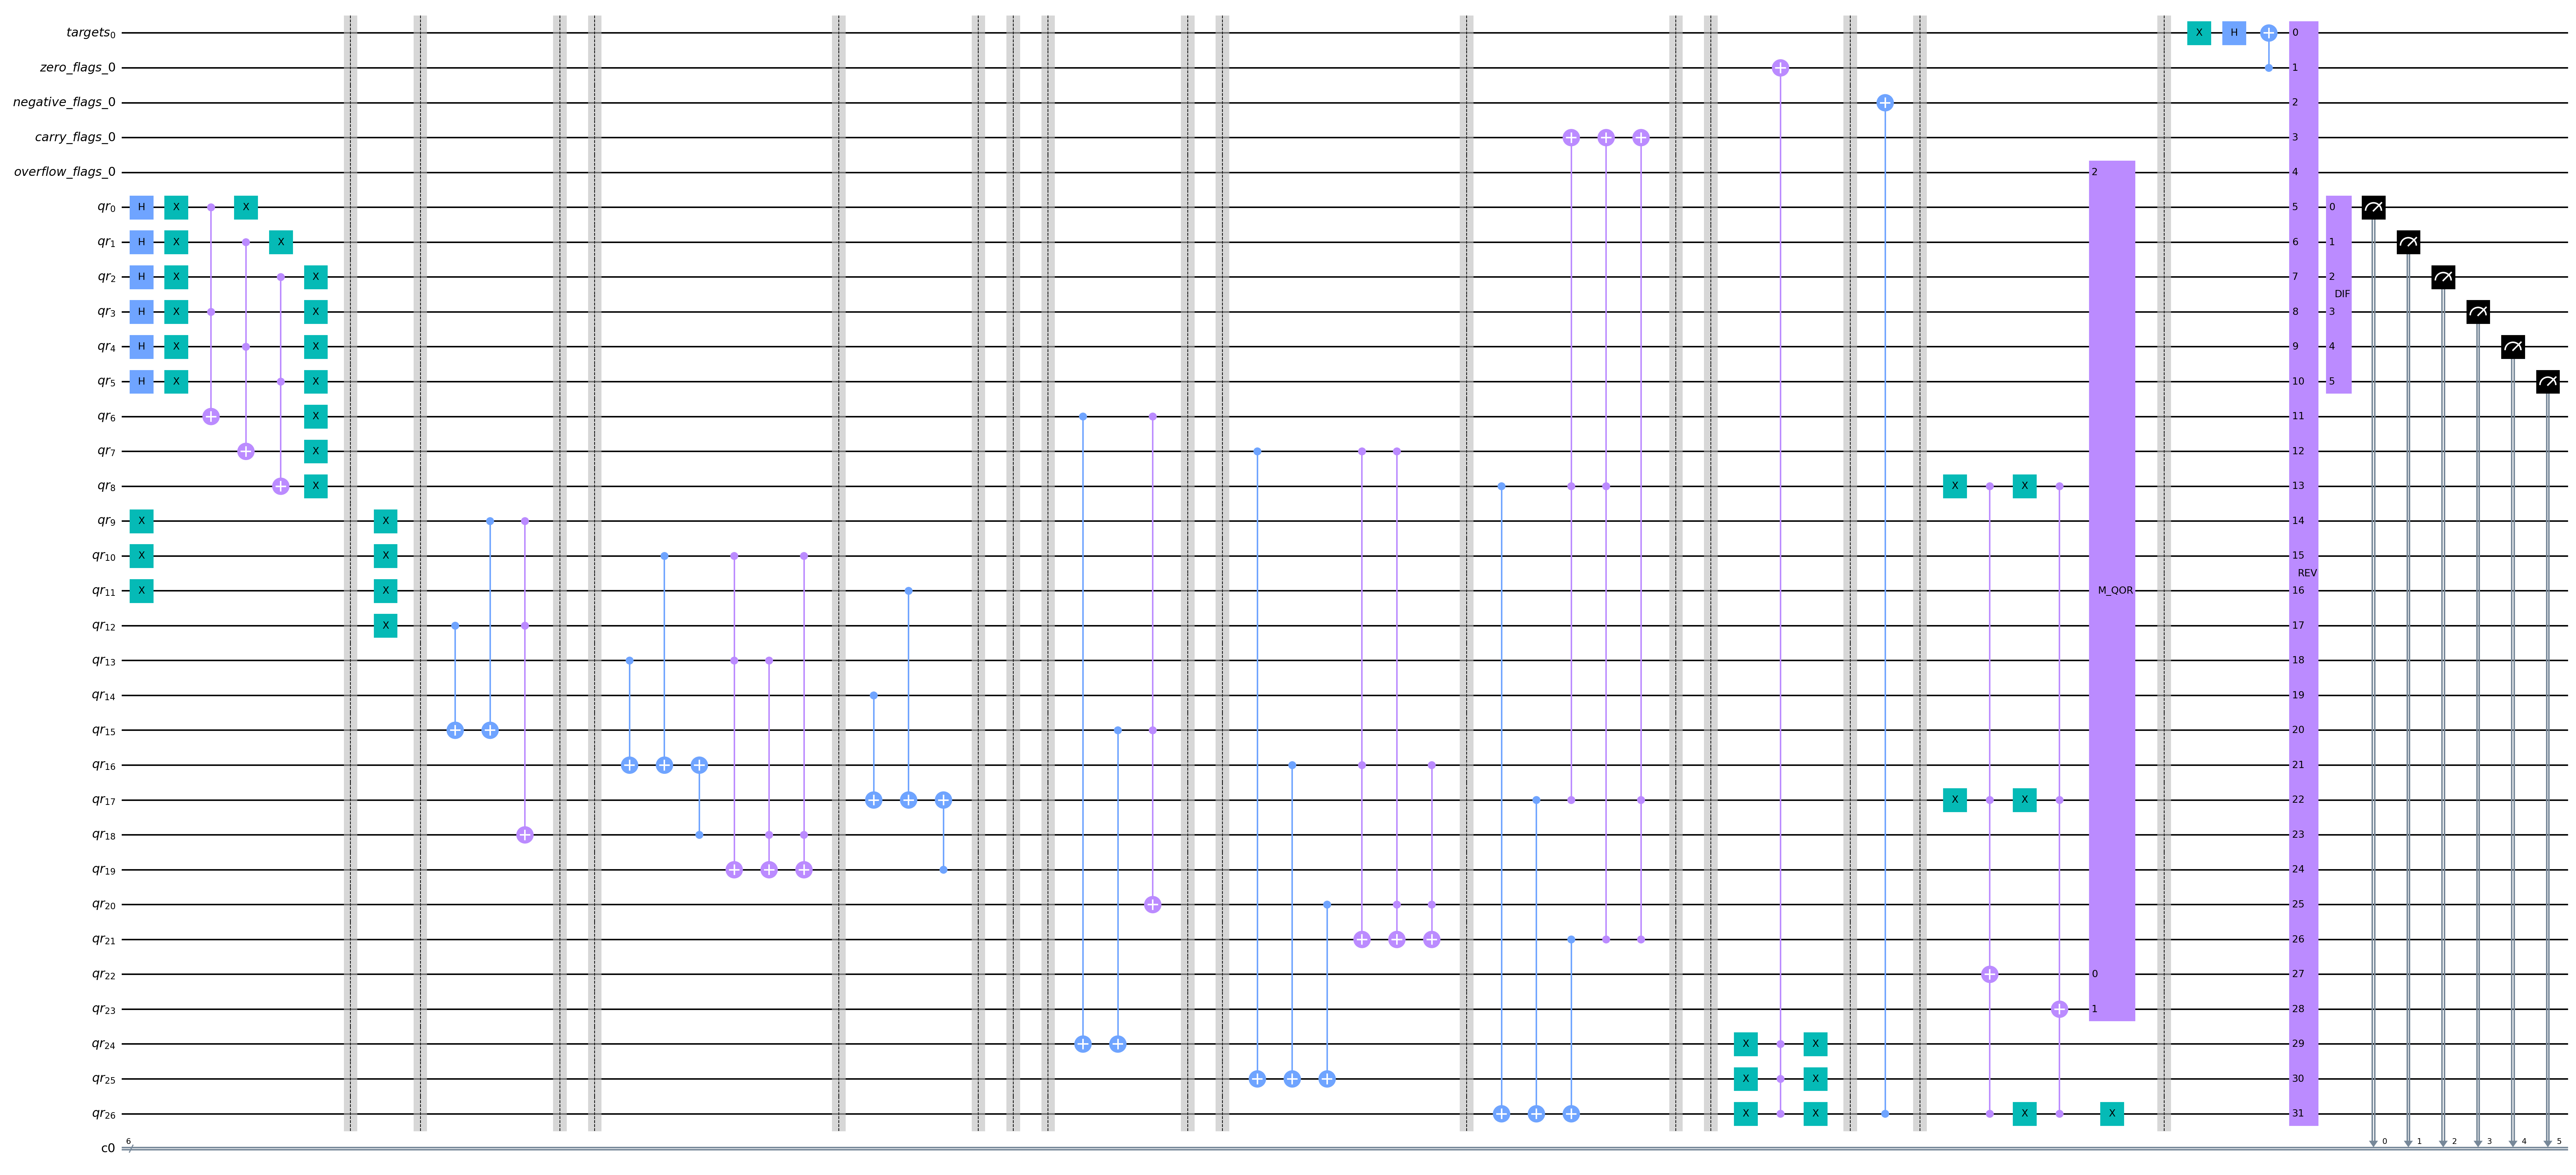
\includegraphics[width=9cm]{Figures/Set_Cover_circuit.png}
    \caption{Using Grover's Algorithm to Solve the Set Cover Problem}
    \label{fig:Set_Cover}
\end{figure}

\section{Conclusion}
In this paper, we have presented a novel quantum algorithm for solving the Set Cover problem using Grover's Algorithm. Our approach leverages the inherent speed-up of Grover's Algorithm to efficiently search the solution space of the Set Cover problem, providing a more scalable alternative to classical algorithms. Our proposed algorithm has the potential to bring significant benefits to various application domains, including resource allocation, network design, and computational biology, where the Set Cover problem plays a crucial role.

While our research presents a promising step towards addressing the computational challenges of the Set Cover problem using quantum computing, several avenues for future research remain. One direction for future work could involve the exploration of alternative quantum algorithms and techniques to further improve the efficiency and scalability of our approach. Additionally, the development of quantum hardware and software platforms capable of executing our algorithm in practice will be essential to realize its full potential.

In conclusion, our research contributes to the growing body of work exploring the application of quantum computing techniques to combinatorial optimization problems. We hope that our results will inspire further research in this area and ultimately lead to the development of more efficient and practical solutions for the Set Cover problem and other challenging computational problems.

